\documentclass[xcolor=dvipsnames]{beamer}
%%%%%%%%%%%%%%%%%%%%%%%%%%%%%%%%%%%%
%
% Packages
%
%%%%%%%%%%%%%%%%%%%%%%%%%%%%%%%%%%%%
\usepackage{hyperref}
\usepackage{caption}
\usepackage{subcaption}
\usepackage{amsmath,amsfonts,amssymb}
\usepackage{lmodern}
\usepackage{graphicx}
\usepackage{caption}
\setcounter{MaxMatrixCols}{14}
\usepackage{multicol}
\usepackage{etoolbox}
\usepackage{bibentry}
\usepackage{dsfont}

\usepackage[utf8]{inputenc}
\usepackage[T1]{fontenc}
\usepackage[french]{babel}

\usepackage{babel,blindtext}
\usepackage{color}
\DeclareMathOperator*{\argmin}{arg\,min}
\usepackage{tikz}
\usetikzlibrary{shapes,shadows,arrows}

\setbeamercovered{dynamic}
\useinnertheme{rectangles}


%%%%%%%%%%%%%%%%%%%%%%%%%%%%%%%%%%%%
%
% Theme
%
%%%%%%%%%%%%%%%%%%%%%%%%%%%%%%%%%%%%
\usetheme{Boadilla}
\usecolortheme[named=Brown]{structure}
\usetheme[height=7mm]{Rochester}

\title{Coalition Formation Algorithm of Prosumers in a Smart Grid Environment}
\author[N. Gensollen]{\textbf{Nicolas Gensollen}, Vincent Gauthier, Monique Becker, Micher Marot}
\institute[TSP]{
  CNRS SAMOVAR, Telecom SudParis\\
  Institut Mines\-Telecom\\[1ex]
  \texttt{nicolas.gensollen@telecom-sudparis.eu}
}
\date{16 december 2014, 

{\footnotesize disponible sur ArXiv à : \textit{http://arxiv.org/abs/1410.8776}} }

%%%%%%%%%%%%%%%%%%%%%%%%%%%%%%%%%%%%
%
% Main Document
%
%%%%%%%%%%%%%%%%%%%%%%%%%%%%%%%%%%%%
\begin{document}

%%%%%%%%%%%%%%%%%%%%%%%%%%%%%%%%%%%%
%
% Slides Title
%
%%%%%%%%%%%%%%%%%%%%%%%%%%%%%%%%%%%%
\begin{frame}
	\bibliographystyle{plain}
	\nobibliography{beamer}
		\titlepage
\end{frame}

%%%%%%%%%%%%%%%%%%%%%%%%%%%%%%%%%%%%
%
% Slides Title
%
%%%%%%%%%%%%%%%%%%%%%%%%%%%%%%%%%%%%
\begin{frame}
	\frametitle{Outline}

	\tableofcontents

\end{frame}

%%%%%%%%%%%%%%%%%%%%%%%%%%%%%%%%%%%%
%
% Slide 1
%
%%%%%%%%%%%%%%%%%%%%%%%%%%%%%%%%%%%%
\section{Objective}
\begin{frame}
	\frametitle{Objective}
	
	\begin{small}
	\begin{itemize}
		\item Data/Communication oriented
		\item \textbf{Prosumer} scenario (agents consumme, produce, and sell to the grid)
		\item \textbf{Minimizing} the amount of \textbf{communication} needed to maintain stability
		\item Avoid communication \textbf{bottlenecks}
		\item Organizing prosumers into virtual \textbf{coalitions} (geographical distances are abstracted)
		\item Reduce the "\textit{grid to agents}" type of communication flows
		\item How should these coalitions be formed ?
	\end{itemize}		
	\end{small}
	
	\begin{figure}
		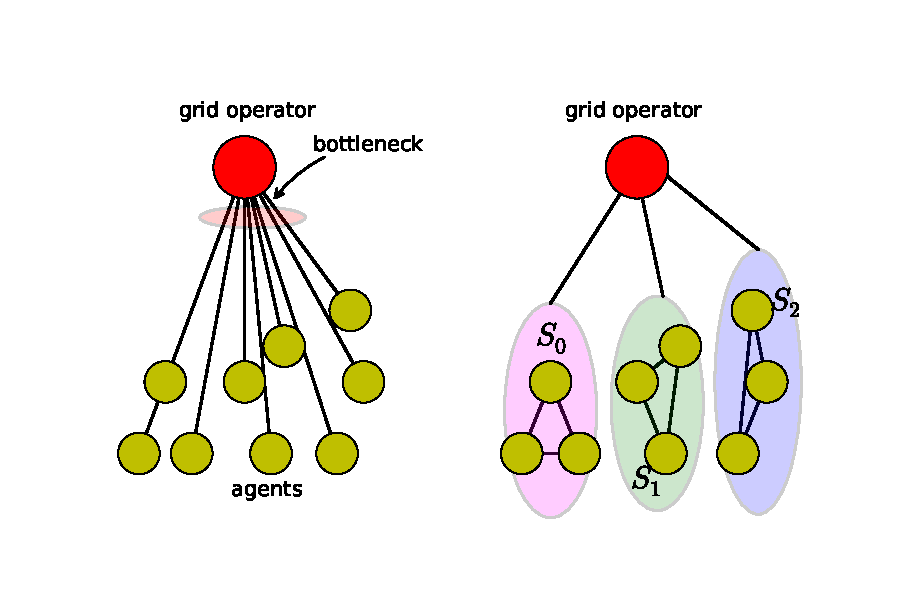
\includegraphics[scale=.4]{coalition_communication.pdf}
	\end{figure}		
	
\end{frame}

%%%%%%%%%%%%%%%%%%%%%%%%%%%%%%%%%%%%
%
% Slide 2
%
%%%%%%%%%%%%%%%%%%%%%%%%%%%%%%%%%%%%
\section{Challenges}
\begin{frame}
	\frametitle{Challenges}
	
	\begin{footnotesize}
	\begin{itemize}
		\item Suppose coalitions are formed \textbf{on day d for day $ d +1 $}
		\item A \textbf{contract value} is decided for each coalition
		\item Over day $ d +1 $, coalition net productions are likely to oscillates because :
			\begin{itemize}
				\item {\scriptsize agents \textbf{consume freely}}
				\item {\scriptsize production is based on \textbf{renewables} (lots of \textbf{uncertainties})}
			\end{itemize}
		\item BUT, for the grid operator, coalition \textbf{productions should remain stable} at their contract values
		\item Coalitions need \textbf{communication} to take actions (battery charge/discharge, load scheding, backup generators)
	\end{itemize}
	\end{footnotesize}
	
	\begin{columns}
		\begin{column}{.7 \linewidth}
			\begin{figure}
				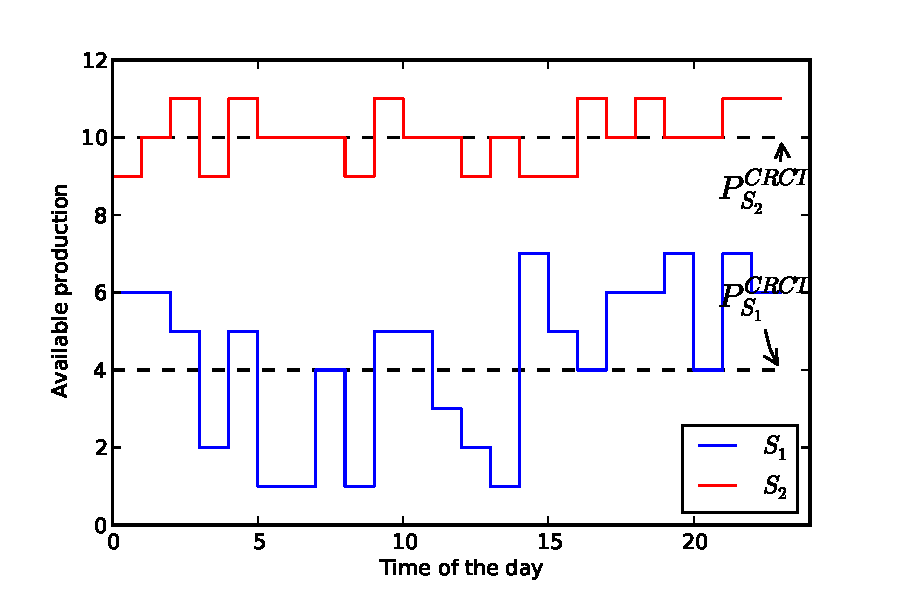
\includegraphics[scale=.38]{production.pdf}
			\end{figure}
		\end{column}
		\begin{column}{.3 \linewidth}
			{\scriptsize We want to minimize the amount of communication needed by forming coalition that, statistically speaking, will be likely to deviate less on day $d+1$ }
		\end{column}
	\end{columns}

\end{frame}
	
%%%%%%%%%%%%%%%%%%%%%%%%%%%%%%%%%%%%
%
% Slide 3
%
%%%%%%%%%%%%%%%%%%%%%%%%%%%%%%%%%%%%
\begin{frame}
	\frametitle{Challenges}
	
	\begin{columns}
		\begin{column}{.5 \linewidth}
			\begin{scriptsize}
			\begin{itemize}			
				\item Agents net production timeseries exhibit \textbf{diverse patterns} because of (mainly):
					\begin{itemize}
						\item {\tiny Weather conditions at the agent location}
						\item {\tiny The DER owned by the agents}
						\item {\tiny The agents consumption habits }
					\end{itemize}
				\item \textbf{Probability distributions} infered from past values
				\item $ \sigma_{ij} = \sqrt{ \sigma_{i}^{2} + \sigma_{j}^{2} + \rho_{ij} \sigma_{i} \sigma_{j} } $
				\item We use the \textbf{Pearson correlation coefficient} to simplify the model
				\item We want to \textbf{cluster} together \textbf{uncorrelated} agents
				\item \textbf{Unusual} and \textbf{complex} objective
			\end{itemize}
			\end{scriptsize}
		\end{column}
		\begin{column}{.5 \linewidth}
			\begin{figure}
				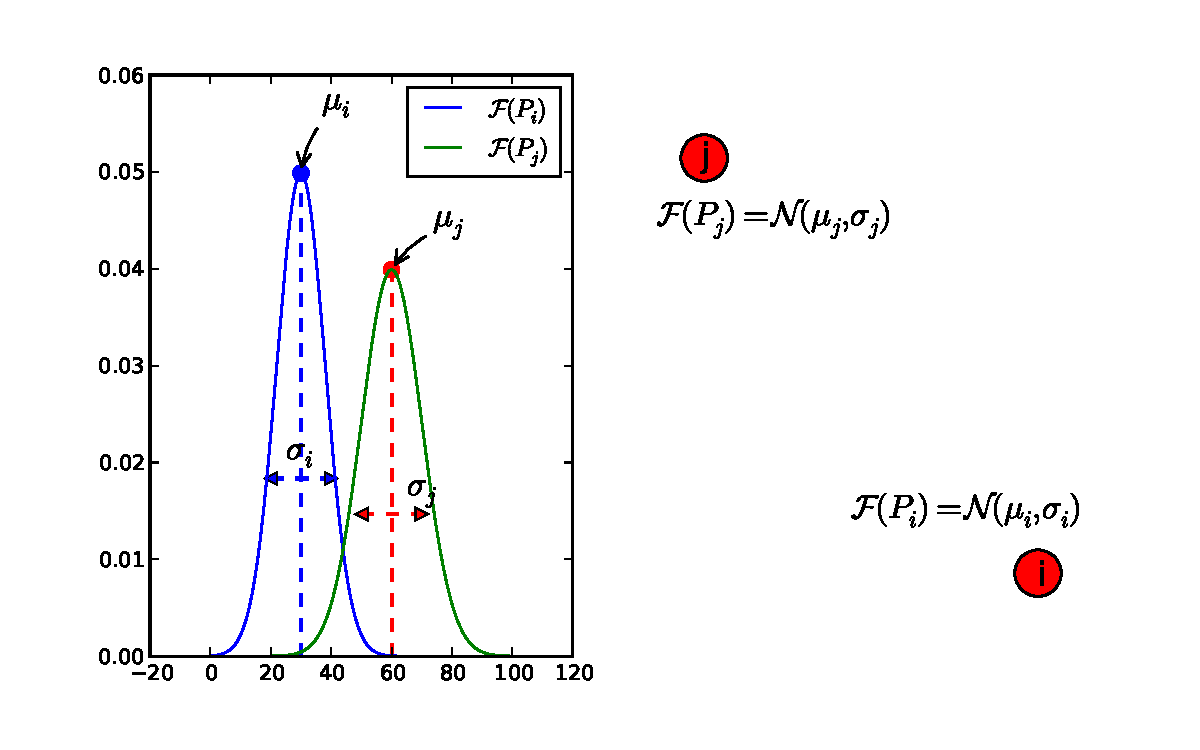
\includegraphics[scale=.25]{example_1.pdf}
			\end{figure}
			\begin{figure}
				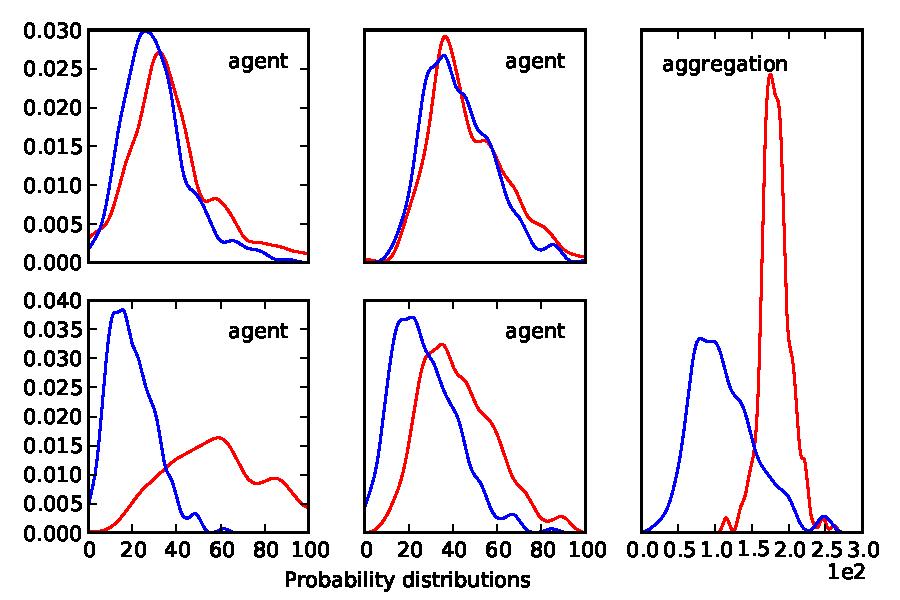
\includegraphics[scale=.3]{distri.pdf}
			\end{figure}
		\end{column}
	\end{columns}

\end{frame}


%%%%%%%%%%%%%%%%%%%%%%%%%%%%%%%%%%%%
%
% Slide 3
%
%%%%%%%%%%%%%%%%%%%%%%%%%%%%%%%%%%%%
\begin{frame}
	\frametitle{Uncorrelated / Diversity Idea}

	\begin{columns}
		\begin{column}{.5 \linewidth}
			\begin{figure}
				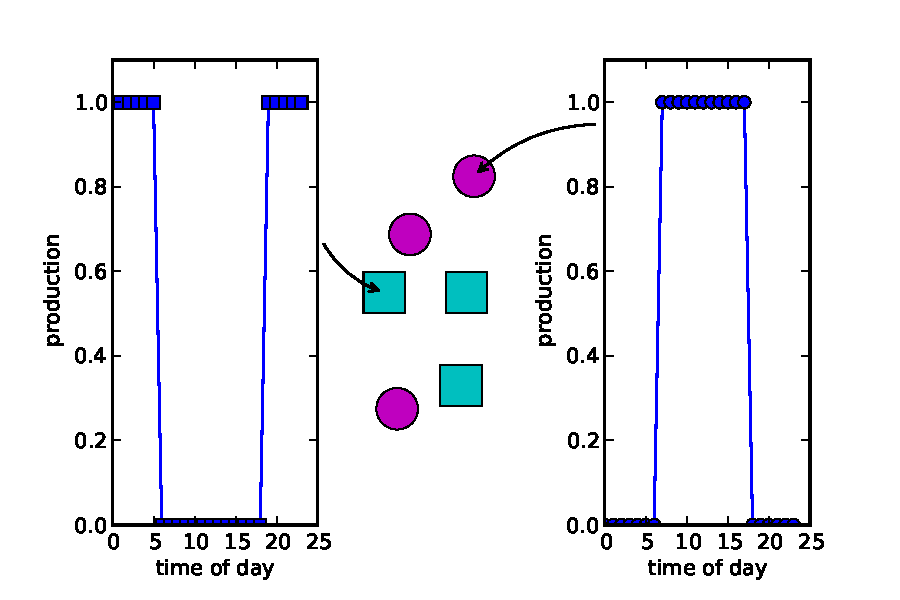
\includegraphics[scale=.4]{rond_carre_1.pdf}
			\end{figure}
		\end{column}
		\begin{column}{.5 \linewidth}
			\begin{figure}
				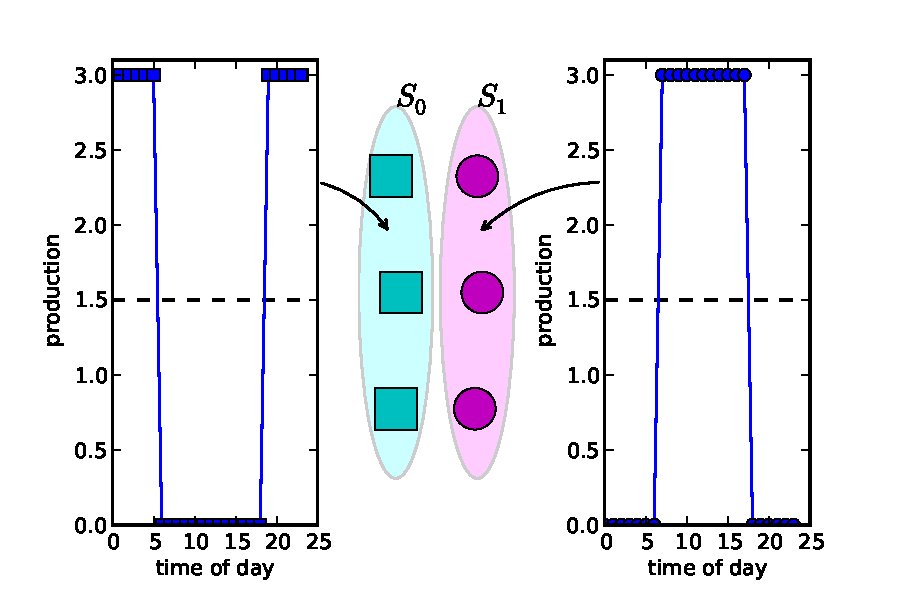
\includegraphics[scale=.35]{rond_carre_2.pdf}
			\end{figure}
			\begin{figure}
				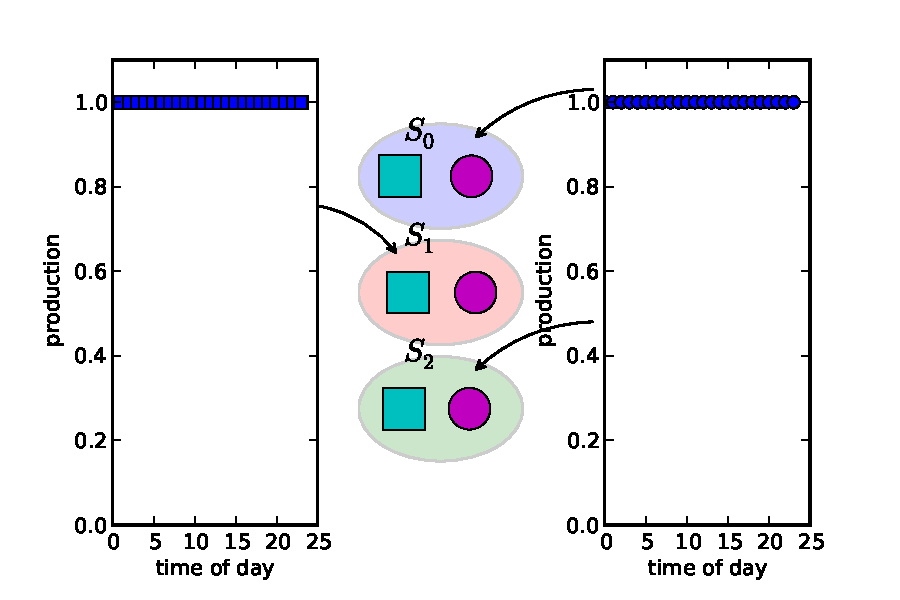
\includegraphics[scale=.35]{rond_carre_3.pdf}
			\end{figure}
		\end{column}
	\end{columns}		
	
\end{frame}

%%%%%%%%%%%%%%%%%%%%%%%%%%%%%%%%%%%%
%
% Slide 4
%
%%%%%%%%%%%%%%%%%%%%%%%%%%%%%%%%%%%%
\section{Data Issues}
\begin{frame}
	\frametitle{Data Issues}
	
	{\small In the model, each agent is represented by the \textbf{timeserie} of its \textbf{net instantaneous production} (production - consumption)	}
	
	\begin{block}{Data}
		\begin{itemize}
			\item {\small Consumption and production data with \textbf{fine granularity}}
			\item {\small Geo-localized data}
			\item {\small "High" sampling frequency (second to hour range)}
		\end{itemize}
	\end{block}		
	
	\begin{itemize}
		\item {\small "Real prosumers" do not really exist yet (necessity to model them)}
		\item {\small We use \textbf{weather data} available for stations accross a given territory}
		\item {\small These traces are used to generate net production traces for prosumer agents (see more details on next slide)}
	\end{itemize}
	
	\begin{figure}
		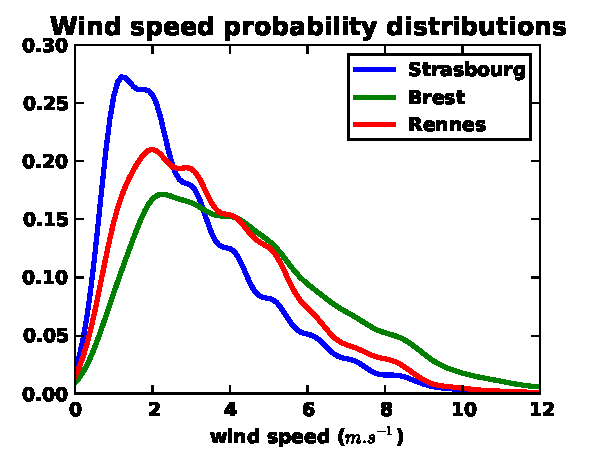
\includegraphics[scale=.3]{wind_distributions.pdf}
		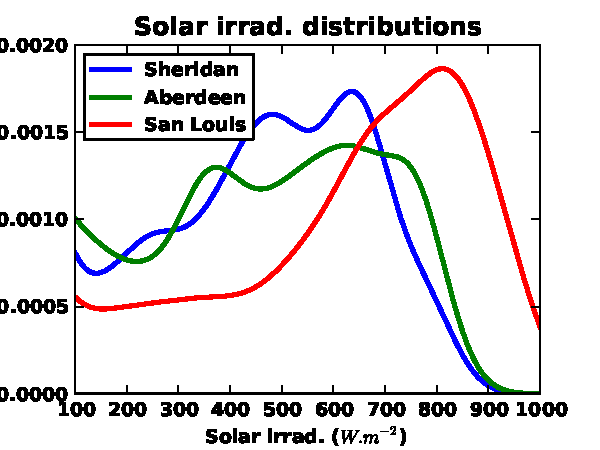
\includegraphics[scale=.3]{solar_distributions.pdf}
	\end{figure}

\end{frame}


%%%%%%%%%%%%%%%%%%%%%%%%%%%%%%%%%%%%
%
% Slides 3
%
%%%%%%%%%%%%%%%%%%%%%%%%%%%%%%%%%%%%
\begin{frame}
	\frametitle{Aggregated net prosumer production model}


\tikzstyle{diams} = [diamond,draw,fill=green!50]
\tikzstyle{line} = [draw,-latex',thick]
\tikzstyle{elli} = [draw, ellipse,fill=red!50, text width = 1em, minimum height=5mm,text centered]
\tikzstyle{block} = [draw,rectangle,fill=blue!50,text width = 3em, minimum height=5mm,text centered]

\begin{tikzpicture}
\node [block](PV){PV};
\node [elli, left of=PV, xshift=-2em](prosumer){i};
\node [block, above of=PV, yshift=1em](eol){Eols};
\node [block, below of=PV, yshift=-1em](conso){$ T_{confort} $};
\node [diams, right of=eol, xshift=2em](F_eol){$\mathcal{F}_{eol}$};
\node [diams, right of=PV, xshift=5em](F_PV){$\mathcal{F}_{PV}$};
\node [diams, right of=conso, xshift=8em](F_conso){$\mathcal{F}_{cons}$};
\node [block, above of=F_PV, yshift=6em](VC){Vec. Climat};
\node [block, right of=F_eol,xshift=8em](P_eol){$P_{i}^{eol}$};
\node [block, right of=F_PV,xshift=5em](P_PV){$P_{i}^{PV}$};
\node [block, right of=F_conso,xshift=2em](C){$C_{i}$};
\node [elli, right of=P_PV, xshift=2em](sum){$\sum$};
\node [block, right of=sum,xshift=2em](P){$P_{i}$};

\path [line](prosumer)-- node[xshift=-0.5em, yshift = 1em]{$N_{eol}$}(eol);
\path [line](prosumer)-- node[xshift=0em, yshift = 0.5em]{$N_{PV}$}(PV);
\path [line](prosumer)--(conso);
\path [line](eol)--(F_eol);
\path [line](PV)--(F_PV);
\path [line](conso)--(F_conso);
\path [line](VC)-| node[xshift=0em, yshift = 0.5em]{$v_{i}$}(F_eol);
\path [line](VC)-- node[xshift=0.5em, yshift = 0.5em]{$e_{i}$}(F_PV);
\path [line](VC)-| node[xshift=0em, yshift = 0.5em]{$T_{i}$}(F_conso);
\path [line](F_eol)--(P_eol);
\path [line](F_PV)--(P_PV);
\path [line](F_conso)--(C);
\path [line](C)--(sum);
\path [line](P_eol)--(sum);
\path [line](P_PV)--(sum);
\path [line](sum)--(P);

%\path [line](graph_complet_b)-- node[xshift=0.5em]{$ \epsilon $} (e_graph_b);
%\path [line](e_graph_b)-- node[xshift=2.8em]{\textit{find cliques}} (seeds_b);
%\path [line](seeds_b)-- node[xshift=2em]{$ \mathcal{U}_{\phi,\ P^{MIN}} $}(over_b);
%\path [line](over_b)-- node[xshift=0.5em]{$ \tau $} (output_b);

%\path [line](decision1)-| node[xshift=1em, yshift = 0.5em]{yes}(process1);
%\path [line](decision1)-| node[xshift=-1em, yshift = 0.5em]{no}(process2);
\end{tikzpicture}

\begin{figure}
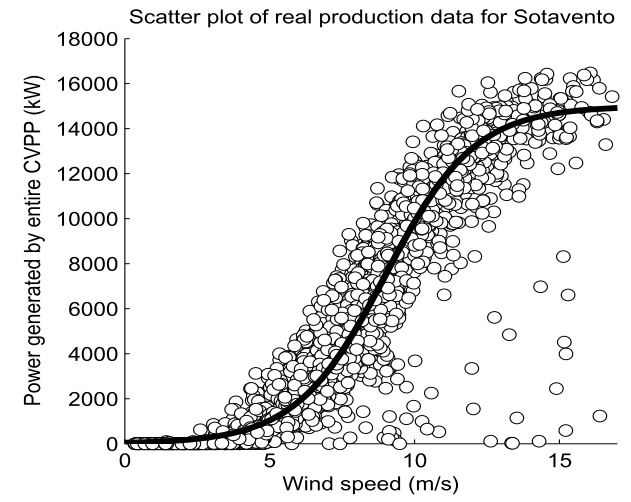
\includegraphics[width=2.5cm]{power_curve.png}
\end{figure}

\end{frame}


%%%%%%%%%%%%%%%%%%%%%%%%%%%%%%%%%%%%
%
% Slide 3
%
%%%%%%%%%%%%%%%%%%%%%%%%%%%%%%%%%%%%
\section{Our Method}
\begin{frame}
	\frametitle{Our Method (Overall view)}
	
	\begin{columns}
		\begin{column}{.6 \linewidth}
			\begin{figure}
				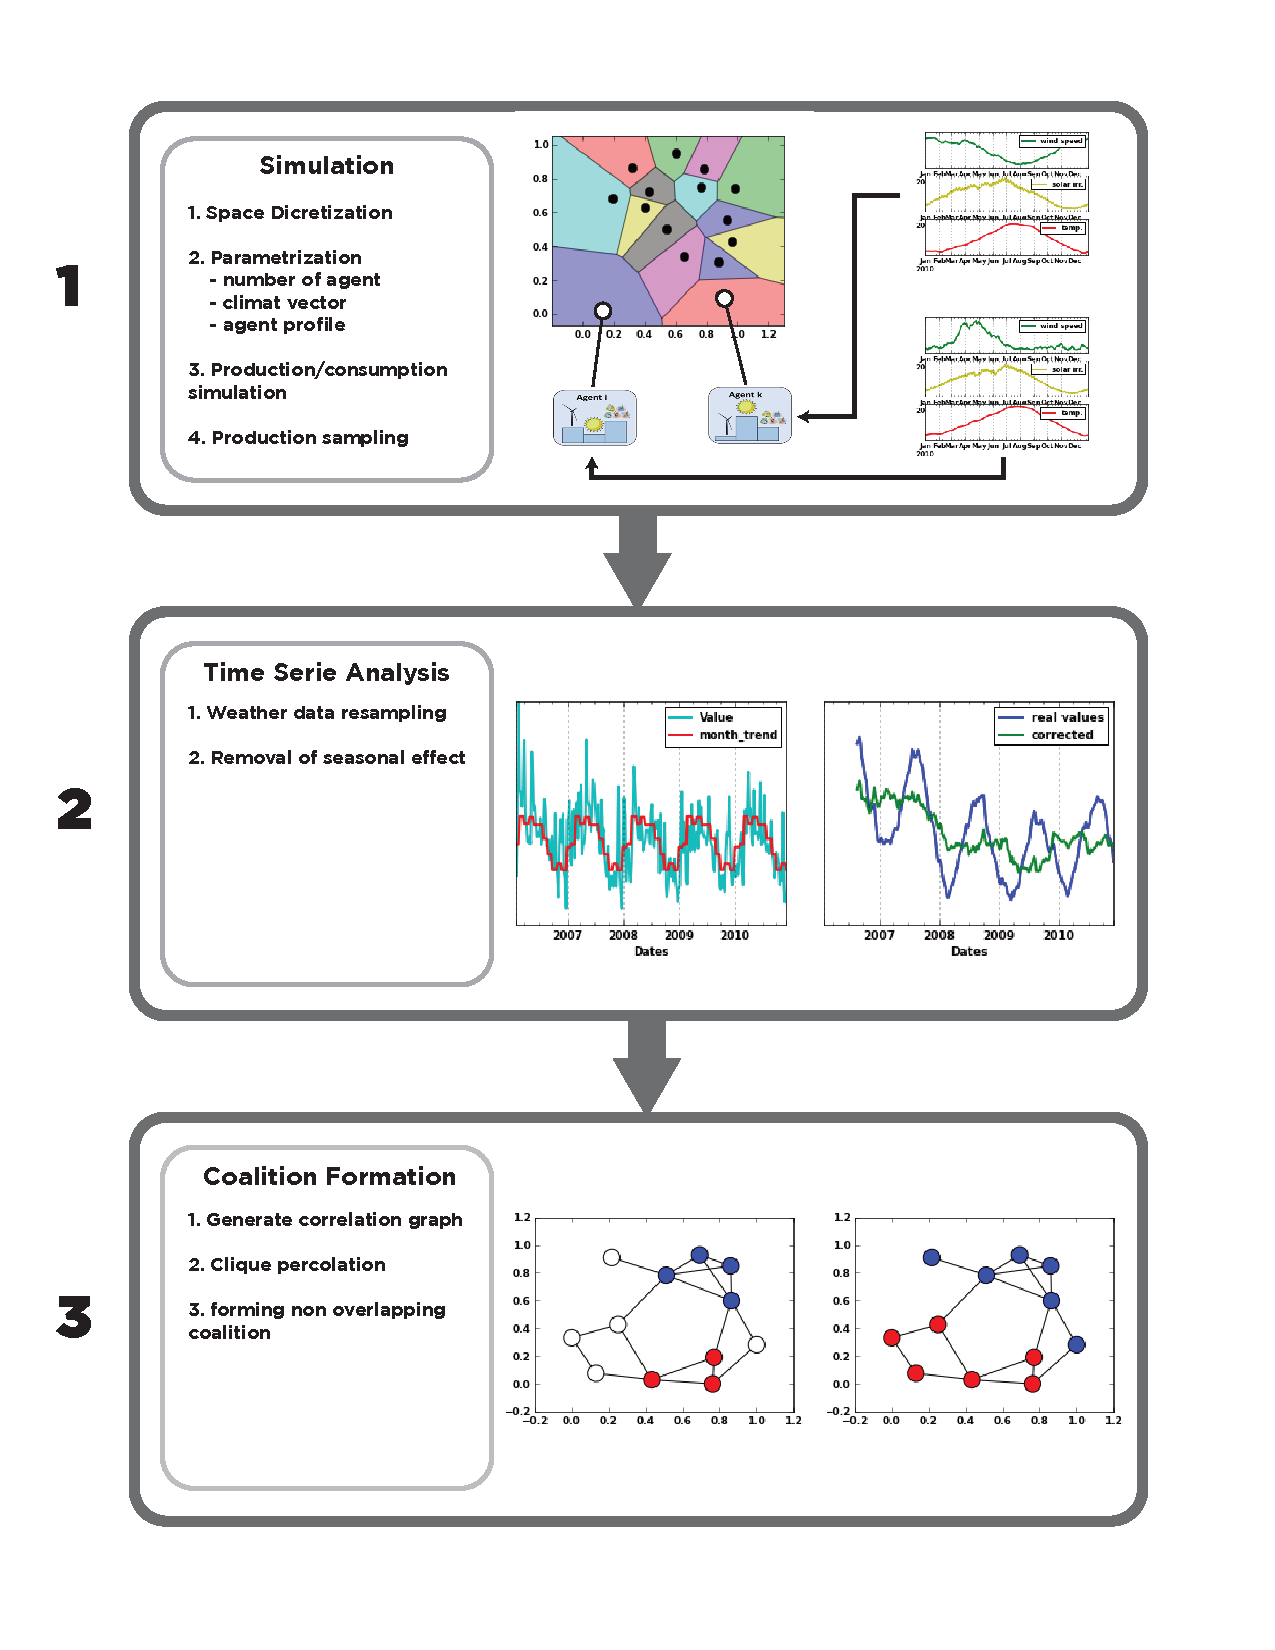
\includegraphics[scale=.3]{Fig2.pdf}
			\end{figure}
		\end{column}
		\begin{column}{.4 \linewidth}
			\begin{itemize}
				\item {\footnotesize Some examples considered :}
				\item {\footnotesize France (Lille, Brest, Dijon, Strasbourg, Bordeaux, Marseille...)}
				\item {\footnotesize USA ( Colorado, Kansas, Montana, Texas, Oklahoma...)}
			\end{itemize}
			\begin{itemize}
				\item {\footnotesize 200 agents}
				\item {\footnotesize 16 zones (16 climate vectors)}
				\item {\footnotesize Timeseries from 01/01/2006 to 31/12/2010}
			\end{itemize}
		\end{column}
	\end{columns}

\end{frame}

%%%%%%%%%%%%%%%%%%%%%%%%%%%%%%%%%%%%
%
% Slide 5
%
%%%%%%%%%%%%%%%%%%%%%%%%%%%%%%%%%%%%
\section{Some Results}
\begin{frame}
	\frametitle{Some Results (part 1)}
	
	\begin{figure}
		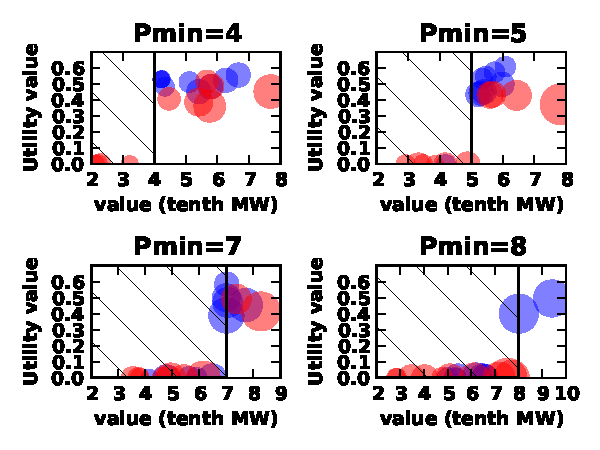
\includegraphics[scale=.5]{coals.pdf}
		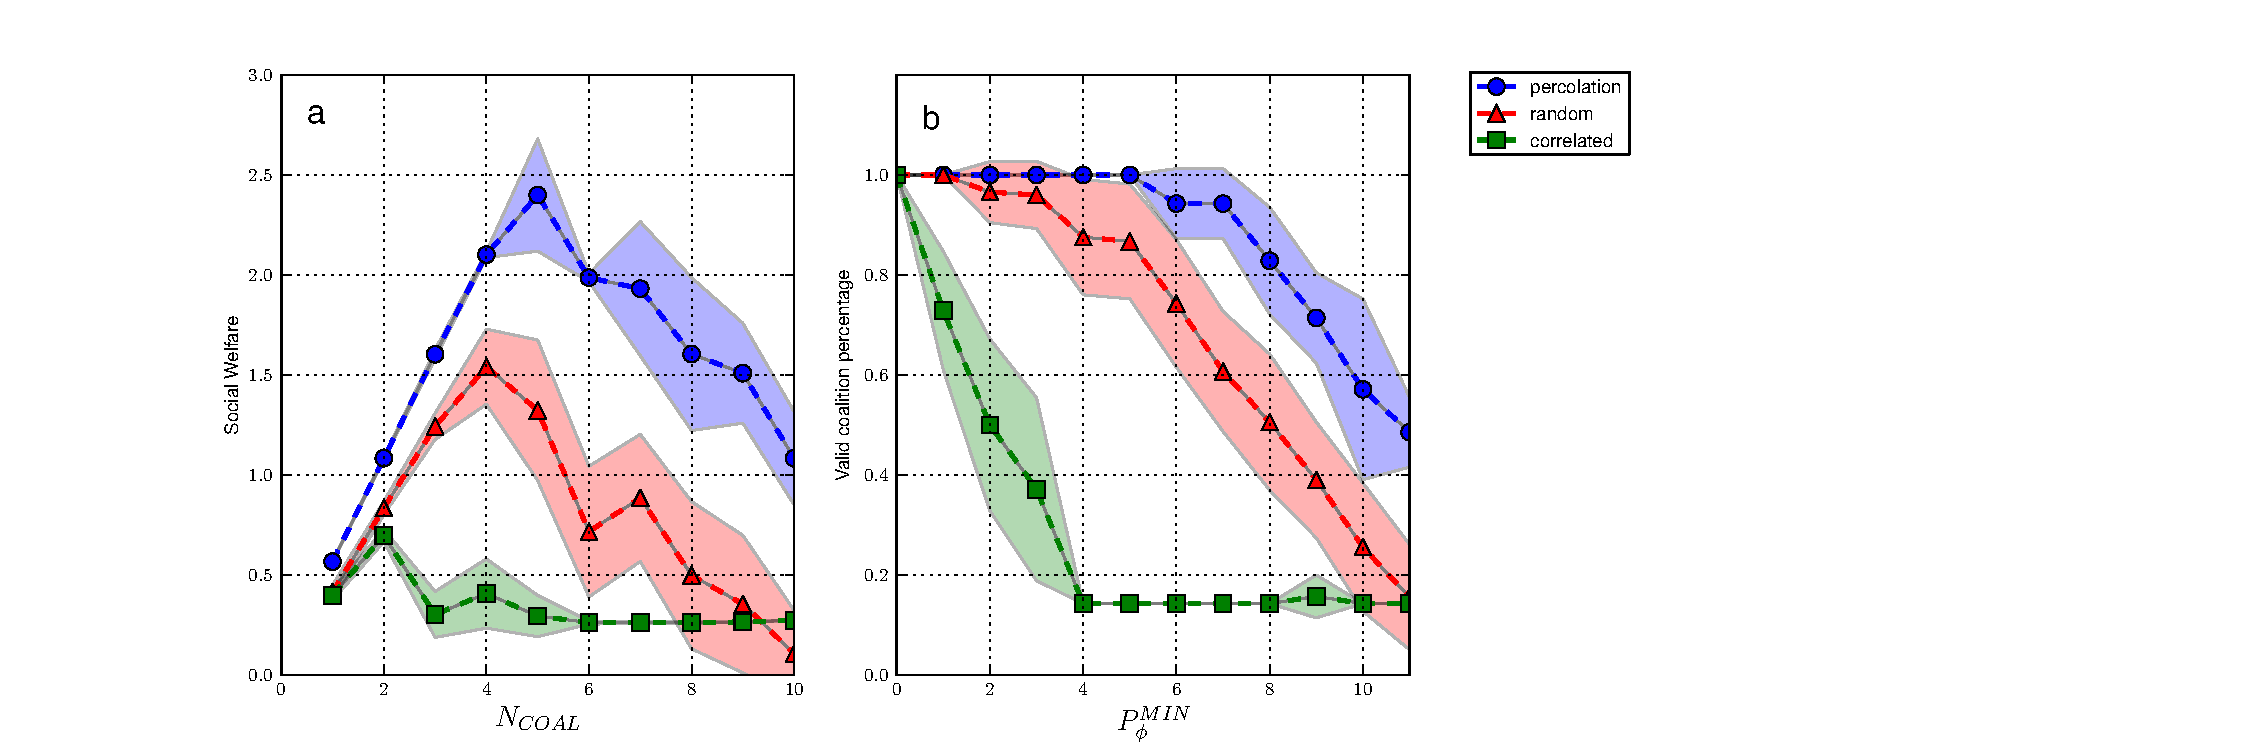
\includegraphics[scale=.3]{fig8.pdf}
	\end{figure}

	\begin{itemize}
		\item {\small Coalitions are able to sell (positive utility) if }
			\begin{itemize}
				\item {\footnotesize They produce more than $ P_{min} $}
				\item {\footnotesize With a low probability of producing less than the contract}
			\end{itemize}
	\end{itemize}

\end{frame}

%%%%%%%%%%%%%%%%%%%%%%%%%%%%%%%%%%%%
%
% Slide 5
%
%%%%%%%%%%%%%%%%%%%%%%%%%%%%%%%%%%%%
\begin{frame}
	\frametitle{Some Results (part 2)}
	
	\begin{figure}
		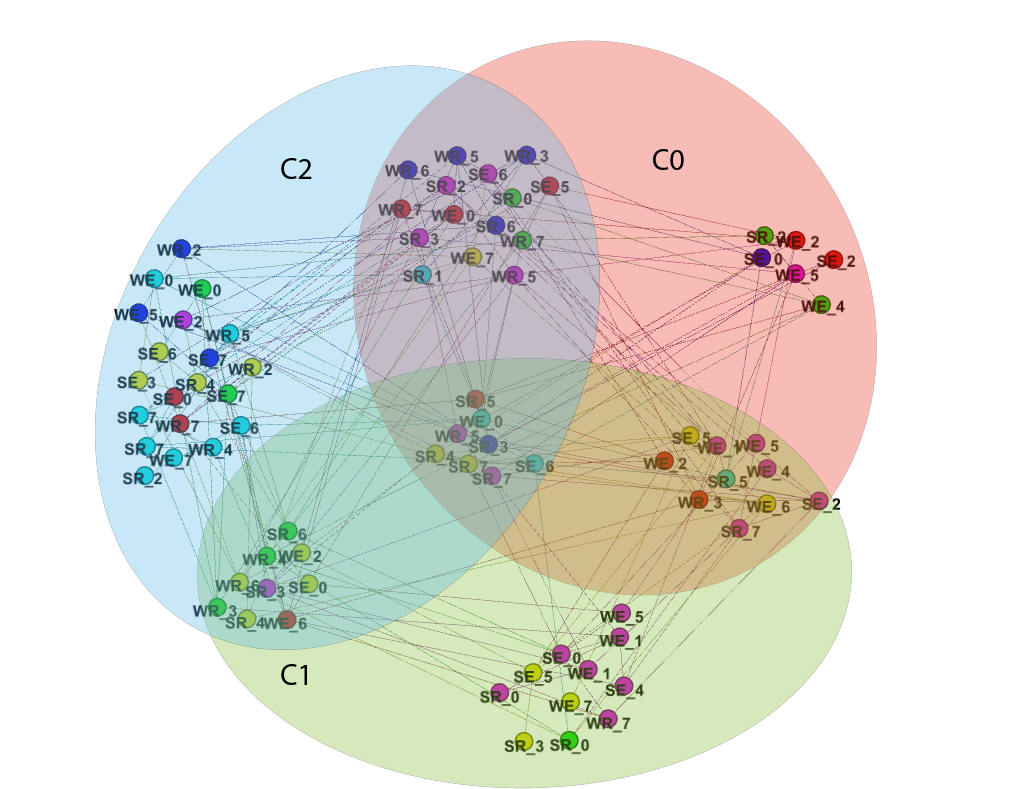
\includegraphics[scale=.15]{Overlap.png}
		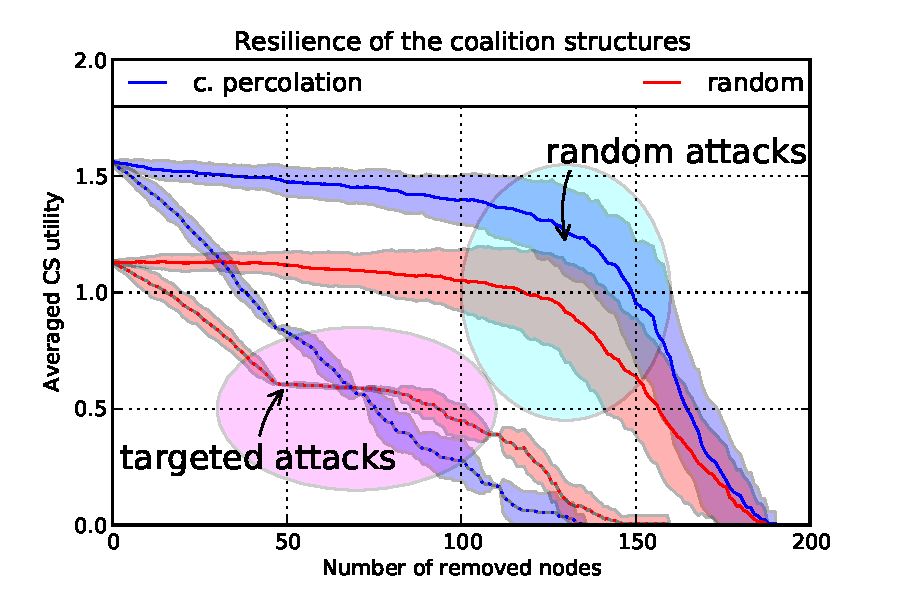
\includegraphics[scale=.35]{resilience_tar_rand.pdf}
	\end{figure}
	
	\begin{figure}
		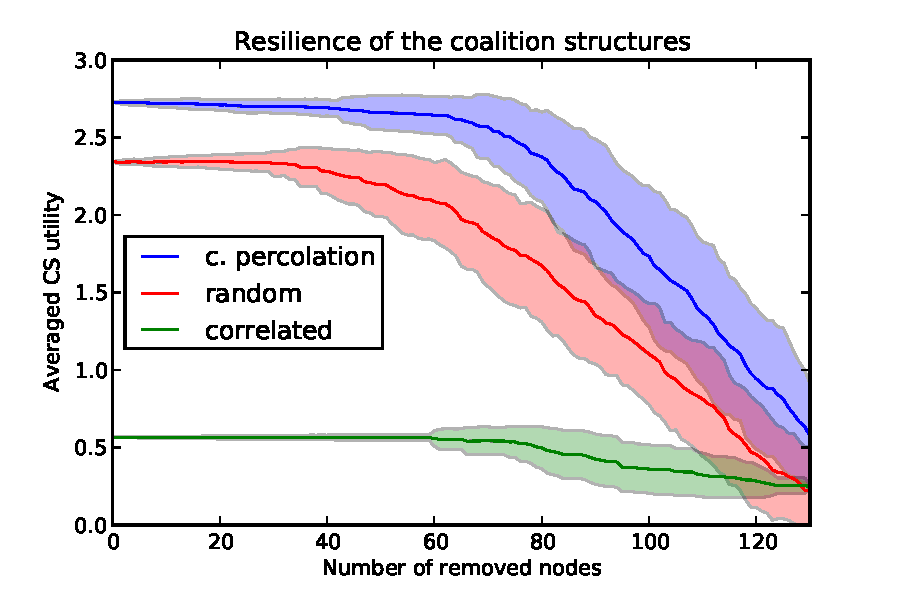
\includegraphics[scale=.35]{resilience_without}
		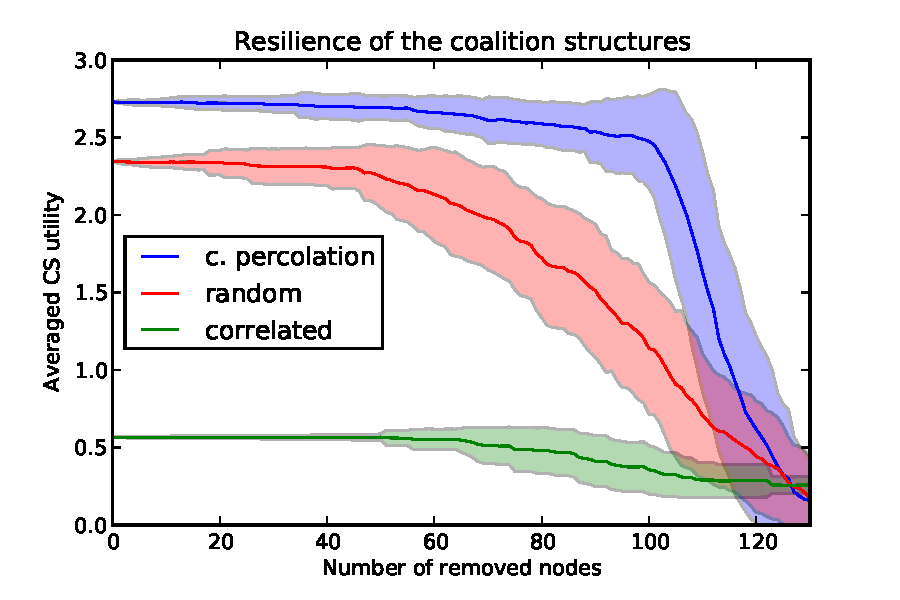
\includegraphics[scale=.35]{resilience_with.pdf}
	\end{figure}

\end{frame}



%%%%%%%%%%%%%%%%%%%%%%%%%%%%%%%%%%%%
%
% Slide 6
%
%%%%%%%%%%%%%%%%%%%%%%%%%%%%%%%%%%%%
\section{Conclusion and Perspectives}
\begin{frame}
	\frametitle{Conclusion and Perspectives}

	\begin{itemize}
		\item Communication oriented
		\item Modeling, simulations
		\item Use of statistical tools, complex systems, graph theory
		\item Lack of available "clean" data led us to construct our own "\textit{traces generator}"
		\item Stong assumptions on the electrical part
		\item Studying the impact of electric constraints on the model could lead to an interesting and more realistic work
	\end{itemize}		
	
\end{frame}


\end{document}
